\chapter{Proiecte similare}

Portable Document Format (PDF) este un tip de fișier dezvoltat de Adobe în anul 1992. La baza acestui fișier stă PostScript, un limbaj de descriere a paginilor. Fiecare document PDF conține o descriere completă a structurii, a textului, a imaginilor și alte informații.

Formatul PDF oferă multe detalii despre fișier. Datorită acestui lucru, nu a fost greu să se creeze aplicații de convertire a documentelor în format HTML. Acestea există de mult timp și folosesc diferite metode pentru a realiza transformarea. În continuare, vom prezenta câteva dintre aceste metode, dar și motivele pentru care nu sunt adecvate în raport cu cerințele noastre.

Aspectele pe care le căutăm la o astfel de aplicație sunt următoarele: fișierul HTML final să aibă textul selectabil, paginile să fie responsive, codul să fie scris într-un mod ușor de editat.


\section{Conversia în imagini}

Una dintre primele soluții luate în considerare este transformarea paginilor din documente PDF în imagini, urmată de inserarea acestora în fișierele HTML. Această metodă este simplă și eficientă din punct de vedere al implementării, dar nu îndeplinește cerințele noastre, deoarece textul nu poate fi selectat.

Pe lângă acest dezavantaj, mai apare și problema dimensiunii imaginilor. Dacă pentru fiecare pagină se salvează câte o imagine, atunci folderul director ar putea să depășească limita maximă admisă din caietul de sarcini dat de Minister.
\begin{figure}[H]
	\centering
	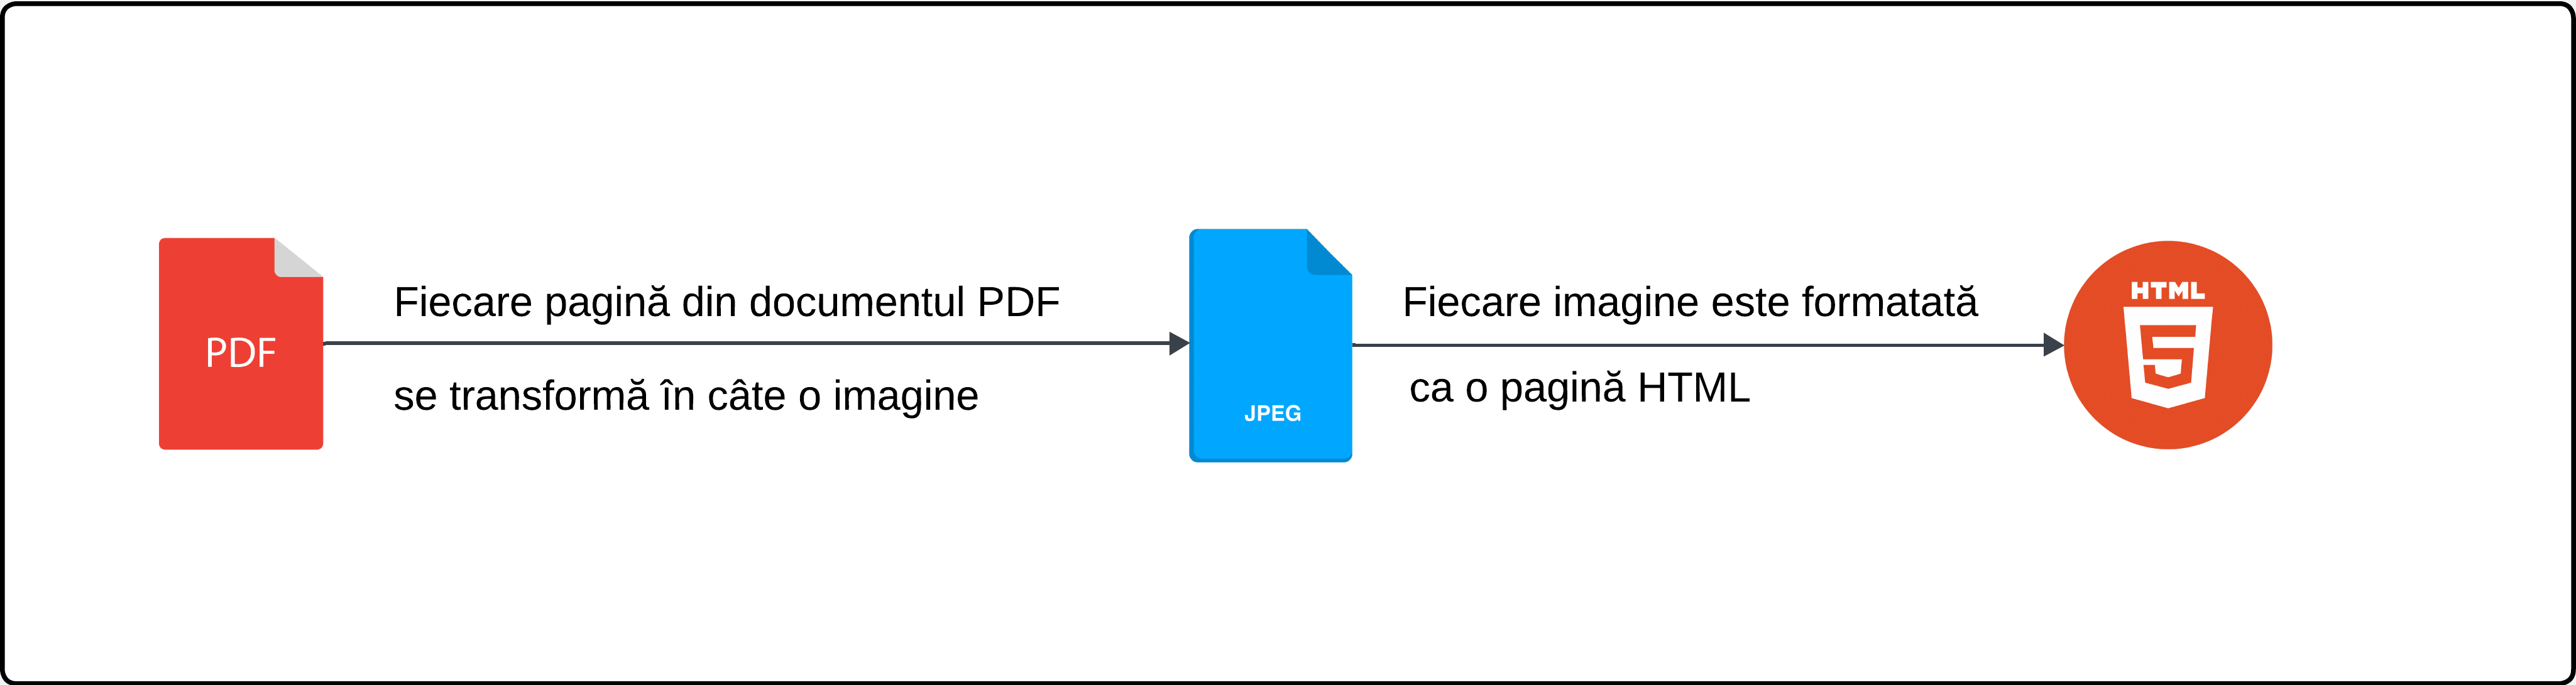
\includegraphics[scale=.40]{Figura2_1}
	\caption{Procesul de transformare al documentului PDF prin transformarea în imagini}
	\label{fig:Figura2_1}
\end{figure}


\section{Soluția de la Adobe Acrobat Pro}

Adobe Acrobat \cite{padova2008adobe} este un software dezvoltat de Adobe, utilizat în toată lumea pentru crearea, manipularea, printarea și gestionarea documentelor PDF.

Una dintre funcționalitățile pe care le are Adobe Acrobat este conversia documentelor PDF în format HTML. Din păcate, această opțiune este disponibilă doar pentru varianta cu plată a software-ului, și anume Adobe Acrobat Pro. Abonamentul lunar pentru acest produs este de 23,79€/lună. Scopul nostru este să găsim o soluție cât mai accesibilă.


\section{XHTML 1.0 Transitional}

Extensible HyperText Markup Language (XHTML) \cite{musciano2006html} este un limbaj folosit pentru crearea și afișarea paginilor web. Acesta este foarte similar cu HTML (HyperText Markup Language), dar include câteva restricții suplimentare. XHTML este o versiune de HTML bazată pe formatul XML, care nu permite, de exemplu, lăsarea tagurilor deschise.

Xodo este un tool care transformă PDF-uri în format XHTML. Acesta permite o singură conversie gratuită pe zi și nu oferă rezultate bune. Structura documentului se desparte în bucăți și nu respectă culoarea de fundal.
\begin{figure}[H]
	\centering
	\begin{subfigure}{.5\textwidth}
		\centering
		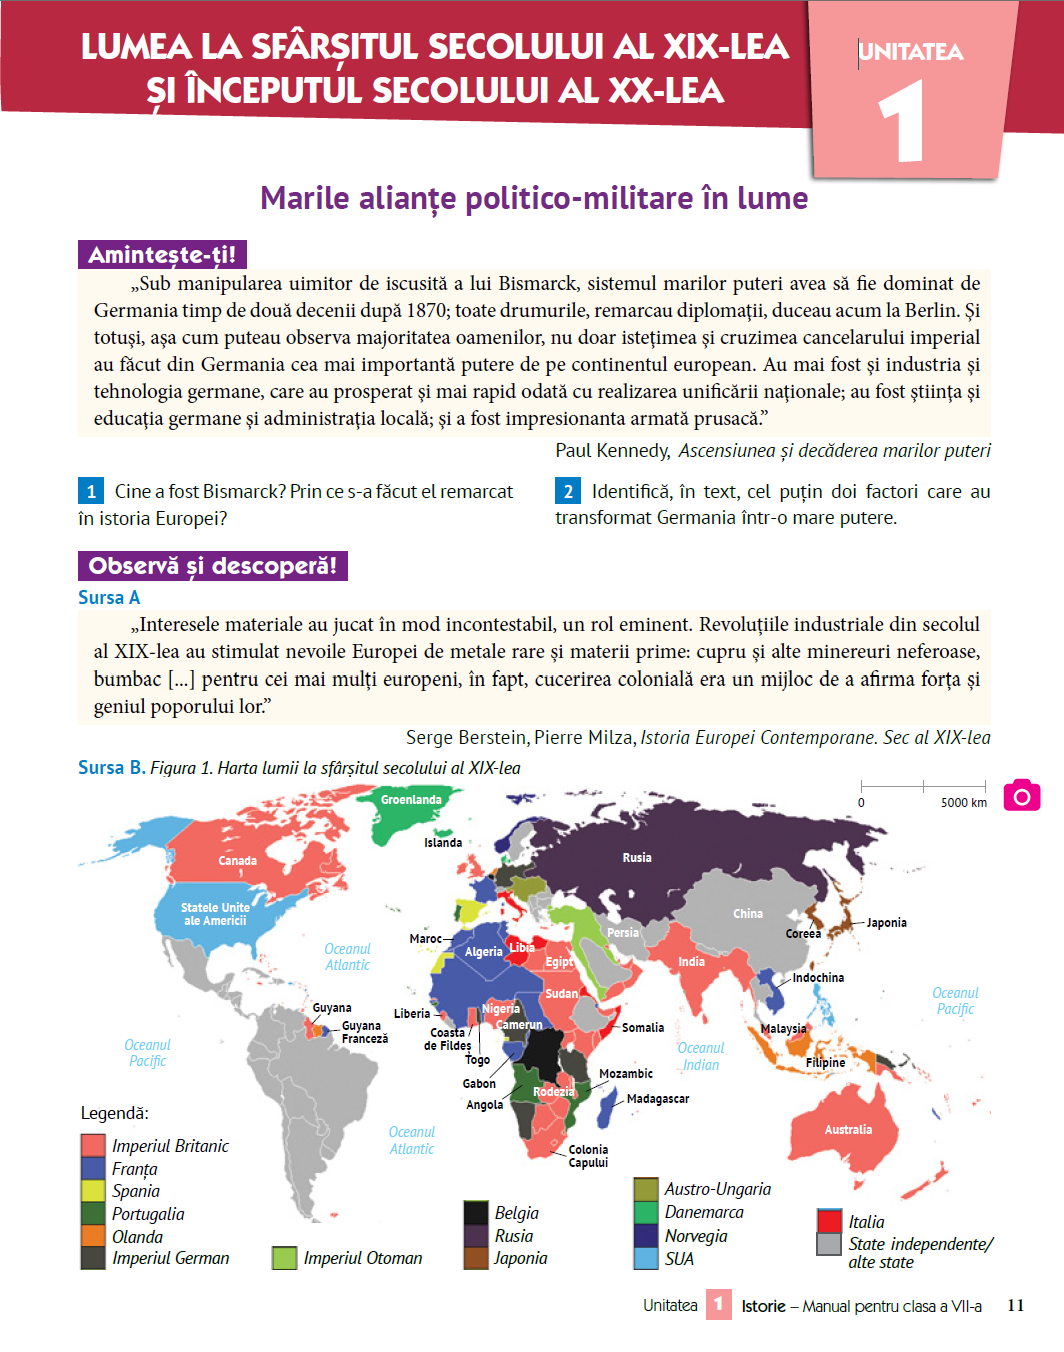
\includegraphics[width=.8\linewidth, height=.30\textheight]{Figura2_2a}
		\caption{pagină din manualul tipărit}
		\label{fig:Figura2_2a}
	\end{subfigure}%
	\begin{subfigure}{.5\textwidth}
		\centering
		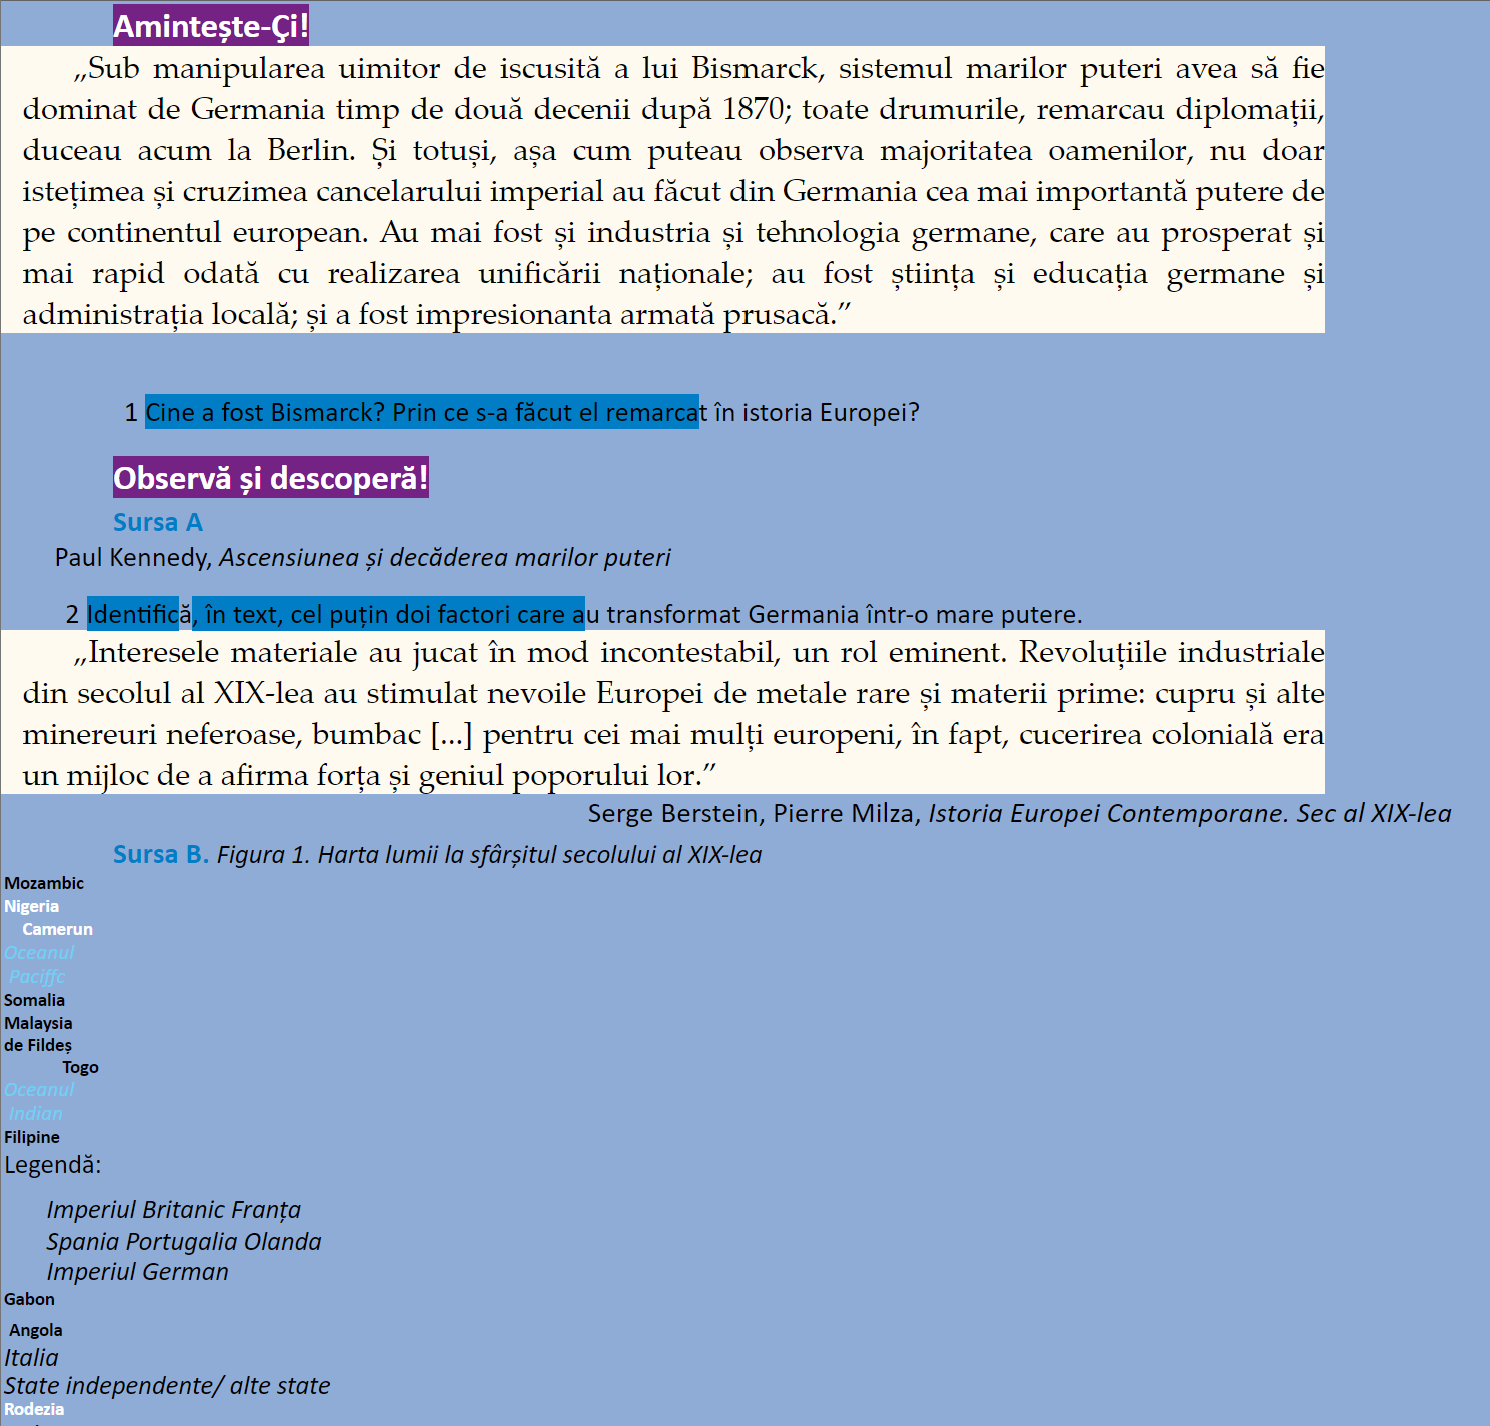
\includegraphics[width=.8\linewidth, height=.30\textheight]{Figura2_2b}
		\caption{pagină HTML generată de Xodo}
		\label{fig:Figura2_2b}
	\end{subfigure}
	\caption{Comparație de pagini dintre varianta tipărită și cea de la Xodo}
	\label{fig:Figura2_2}
\end{figure}

O soluție care oferă o formatare perfectă este obținută folosind pdf2htmlEX \cite{wang2013online}. Acest tool păstrează tot textul și formatarea din PDF, dar are două dezavantaje. În primul rând, paginile rezultate nu sunt responsive, ceeea ce este o condiție obligatorie. O pagină responsive își păstrează structura atunci când este redimensionată. De exemplu, pagina HTML redimensionată pentru un ecran de telefon ar trebui să-și păstreze structura, ceea ce nu se întâmplă. Pe lângă acest lucru, codul HTML este greu de citit și de editat. O linie de cod poate să ajungă chiar și la 60.000 de caractere. În cazul în care apar modificări în manual, acestea vor fi greu de editat.

Două dintre site-urile care folosesc acest tool sunt CloudConvert și Convertio. Acestea dau rezultate asemănătoare, dar au amândouă aceleași probleme.
\begin{figure}[H]
	\centering
	\begin{subfigure}{.5\textwidth}
		\centering
		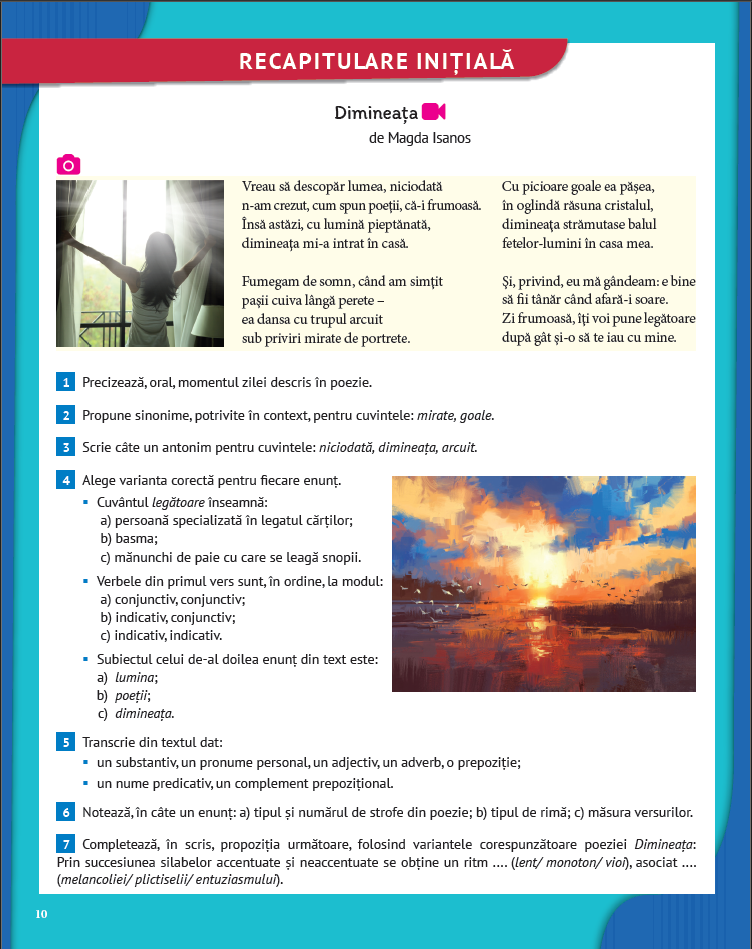
\includegraphics[width=.8\linewidth, height=.30\textheight]{Figura2_3a}
		\caption{pagină din manualul tipărit}
		\label{fig:Figura2_3a}
	\end{subfigure}%
	\begin{subfigure}{.5\textwidth}
		\centering
		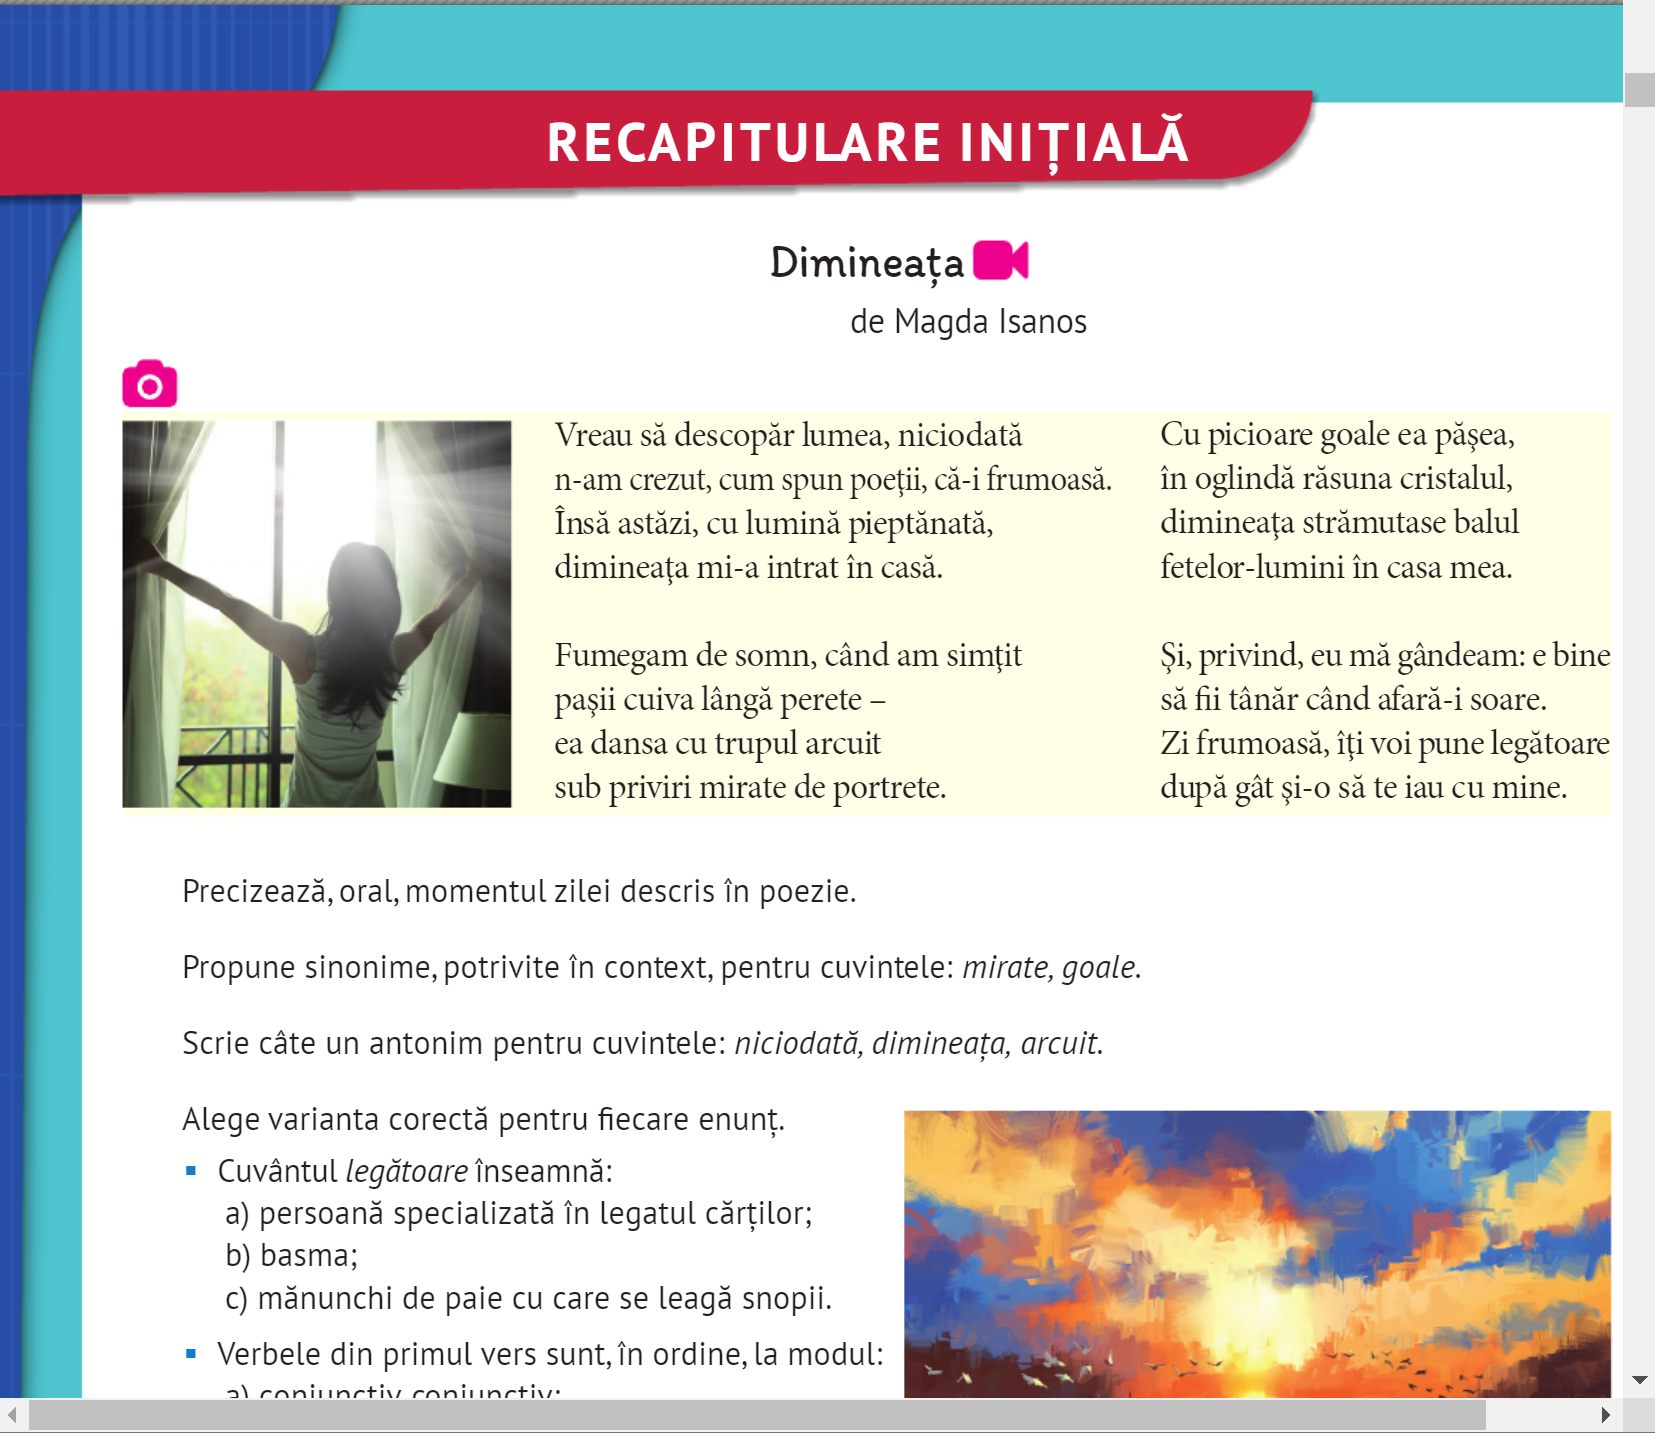
\includegraphics[width=.8\linewidth, height=.30\textheight]{Figura2_3b}
		\caption{pagină HTML generată de CloudConvert}
		\label{fig:Figura2_3b}
	\end{subfigure}
	\caption{Comparație de pagini dintre varianta tipărită și cea de la CloudConvert}
	\label{fig:Figura2_3}
\end{figure}


\section{HTML 4.01 Transitional}

Ultima soluție găsită a fost extragerea textului din documentul PDF și plasarea acestuia într-un fișier de tip HTML 4.01 Transitional \cite{raggett1997html}. Deși acest format este mai simplu de utilizat și editat, el nu este la fel de modern și flexibil ca HTML5.

Un exemplu de site care utilizează această metodă de conversie este PDF24 Tools. Avantajul principal al acestui site este ușurința cu care poți edita codul HTML. Totuși, site-ul nu păstrează formatul original al documentului HTML. Singurele atribute pe care le menține sunt stilurile de text bold și italic.
\begin{figure}[H]
	\centering
	\begin{subfigure}{.5\textwidth}
		\centering
		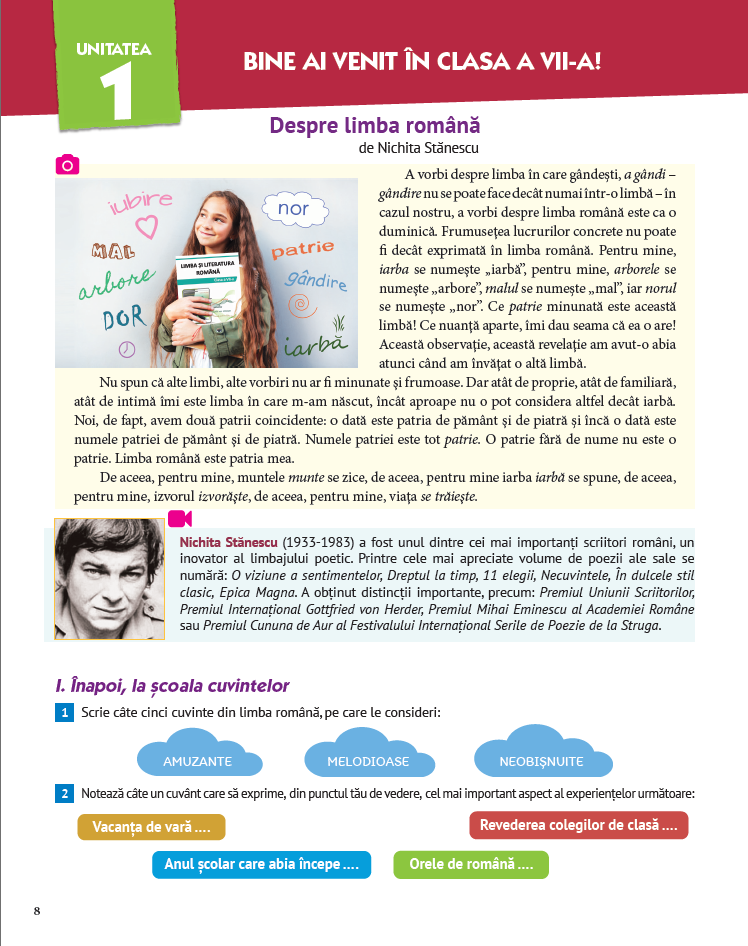
\includegraphics[width=.8\linewidth, height=.3\textheight]{Figura2_4a}
		\caption{pagină din manualul tipărit}
		\label{fig:Figura2_4a}
	\end{subfigure}%
	\begin{subfigure}{.5\textwidth}
		\centering
		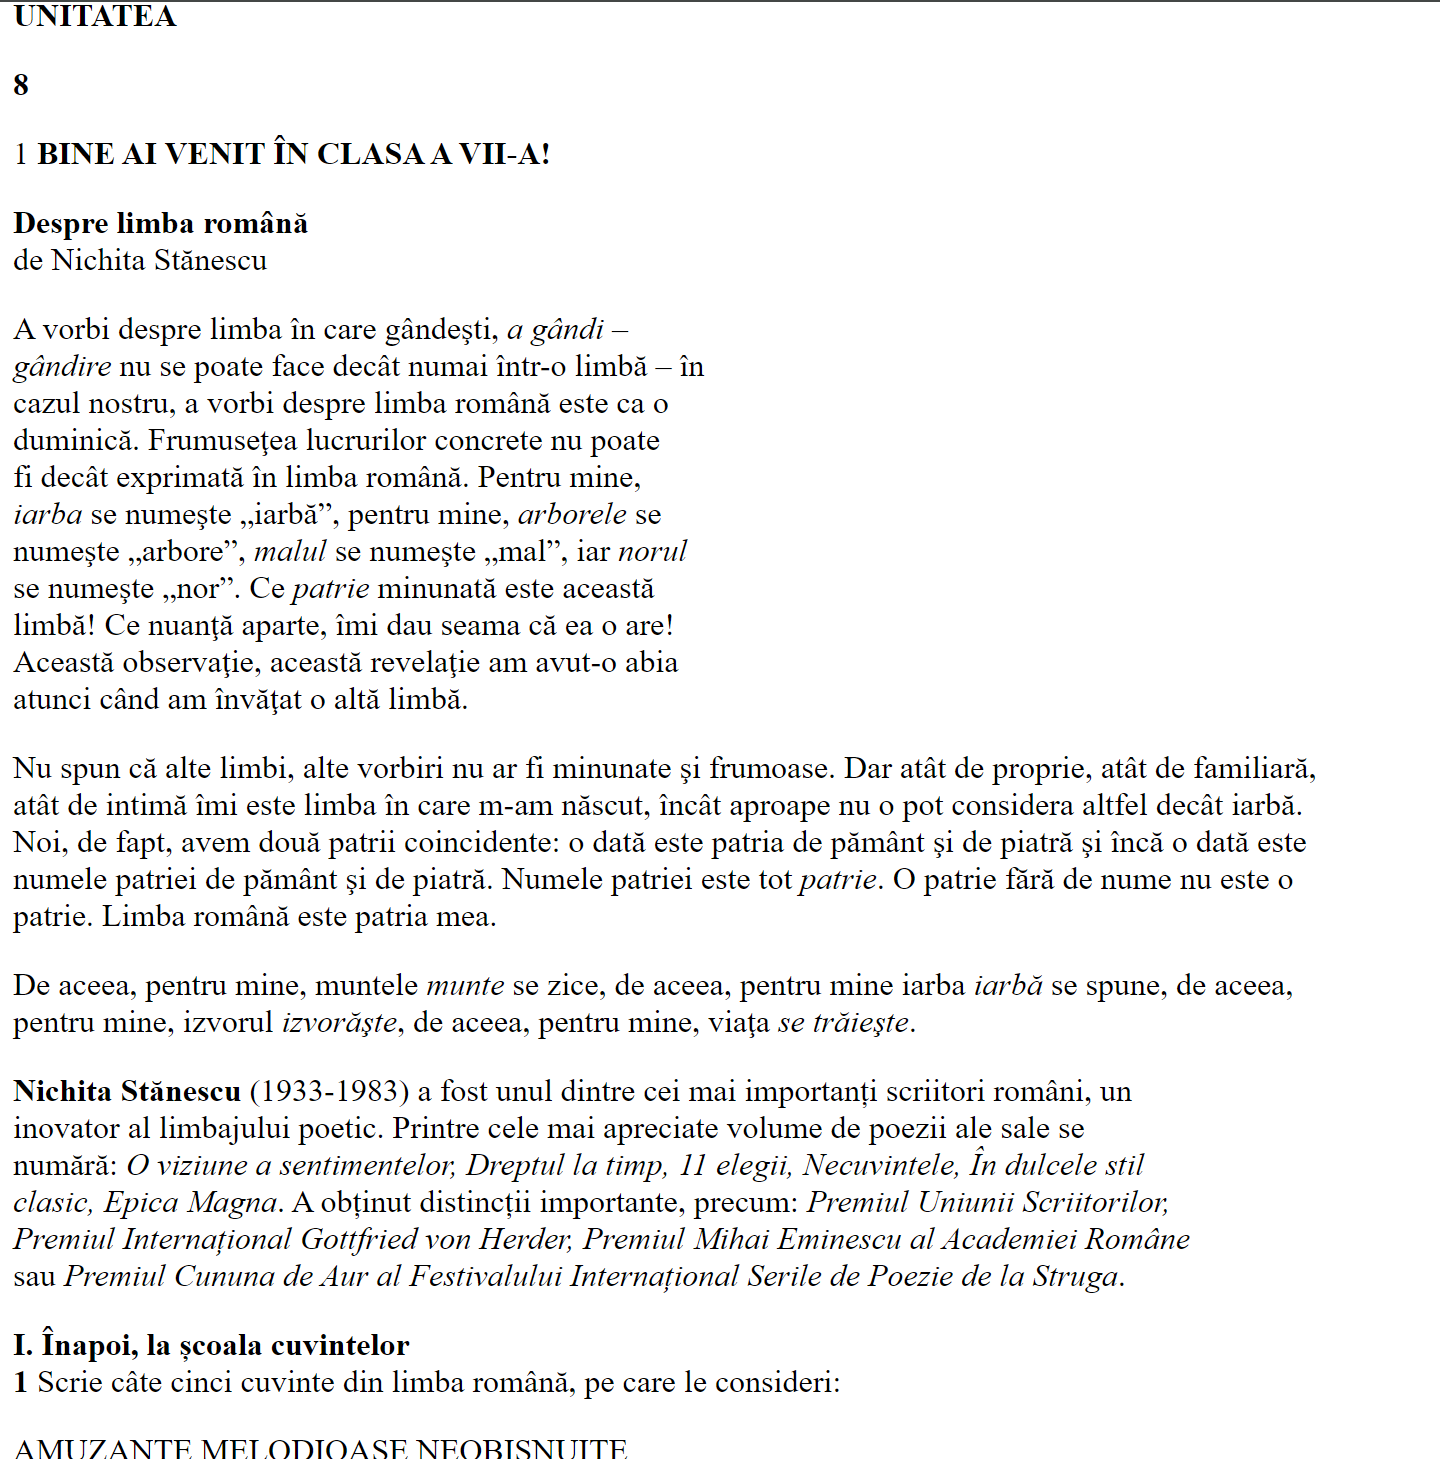
\includegraphics[width=.8\linewidth, height=.3\textheight]{Figura2_4b}
		\caption{pagină HTML generată de PDF24 Tools}
		\label{fig:Figura2_4b}
	\end{subfigure}
	\caption{Comparație de pagini dintre varianta tipărită și cea de la PDF24 Tools}
	\label{fig:Figura2_4}
\end{figure}
\smallskip

Necesitatea de a dezvolta încă un tool de conversie a PDF-urilor în HTML provine din faptul că soluțiile actuale nu satisfac cerințele noastre obligatorii. Mai exact, ne dorim ca textul să fie selectabil, paginile să fie responsive, iar codul HTML să fie ușor de editat. Soluția pe care o propunem va satisface aceste criterii, oferind o alternativă eficientă și constantă.